\documentclass[a4paper,12pt]{article}
\usepackage[utf8]{inputenc}
% Resten af pakkerne
\usepackage[english]{babel}
\usepackage{csquotes}
\usepackage{float}
\usepackage{flafter}
\usepackage{graphicx}
\usepackage{setspace}
\usepackage{enumitem}
\usepackage{multirow}
\usepackage{lmodern}
\usepackage{amssymb,amsmath}
\usepackage{ifxetex,ifluatex}
\usepackage[font=small,labelfont=bf]{caption}
\usepackage{lscape}
\usepackage{xargs}
\usepackage{tabularx}
\usepackage{comment}
\usepackage{pdfpages}
\usepackage{xcolor}
\usepackage{amssymb} 

\usepackage{listings}

\usepackage{ragged2e}

\definecolor{mygreen}{rgb}{0,0.6,0}

\lstnewenvironment{code}[1][]%
{
   \noindent
   \minipage{\linewidth} 
   \vspace{0.5\baselineskip}
   \lstset{language=java, basicstyle=\ttfamily\footnotesize,frame=single,#1}}
{\endminipage}


\lstset{
    stringstyle=\color{mygreen},            % changing string colour to green
    frame=single,                           % adds a frame around the code
    language=Java,                          % the language of the code
    breaklines=true,                        % sets automatic line breaking
    basicstyle=\small,                      % the size of the fonts that are used for the code
    keywordstyle=\color{blue},              % keyword style
    morekeywords={var, UUID, ROLE, EMAIL},  % if you want to add more keywords to the set
    numbers=left,                           % % where to put the line-numbers; possible values are (none, left, right)
    numberstyle=\small,                     % the style that is used for the line-numbers
    commentstyle=\color{mygreen},           % comment style
    captionpos=b,                           % sets the caption-position to bottom
    showstringspaces=false,                 % removes spaces in string
    inputencoding=utf8,
    extendedchars=true,
}

\lstset{literate=%
{æ}{{\ae}}1
{å}{{\aa}}1
{ø}{{\o}}1
{Æ}{{\AE}}1
{Å}{{\AA}}1
{Ø}{{\O}}1
}

% Use for lstlisting formation caption
% \captionsetup[lstlisting]{ format=listing, labelfont=white, textfont=white, singlelinecheck=false, margin=0pt, font={bf,footnotesize}}

% \usepackage[
% backend=biber,
% style=alphabetic,
% sorting=ynt
% ]{biblatex}
% \addbibresource{appendices/bibliography.bib}

% \title{Bibliography management: \texttt{biblatex} package}
% \author{Overleaf}
% \date{ }

\usepackage{ifthen}

\usepackage{xcolor}
% \usepackage{csvsimple}
\usepackage{longtable}

% Margin
\usepackage{geometry}
\geometry{a4paper,  total={170mm,250mm},
 left=20mm,
 top=25mm}


% New Commands
\newcommand\myworries[1]{\textcolor{red}{#1}} 
\newcommand{\myparagraph}[1]{\paragraph{#1}\mbox{}\\}


% Needs to be the last package included
\usepackage{hyperref}
\hypersetup{
    colorlinks=true,
    linkcolor=black,
    filecolor=magenta,      
    urlcolor=blue,
    citecolor=black,
}

\setlength\parindent{0pt} % Removes indent

\begin{document}
    % Removes page numbers
    \pagenumbering{gobble}
    \renewcommand{\thesection}{\Roman{section}} 
    \renewcommand{\thesubsection}{\thesection.\Roman{subsection}}

    \begin{titlepage}
\begin{center}
% Title
{ \LARGE \bfseries Bierproductie \\[0.4cm]}
A Manufacturing Execution System for brewing machines
\begin{figure}[H]
\centering 
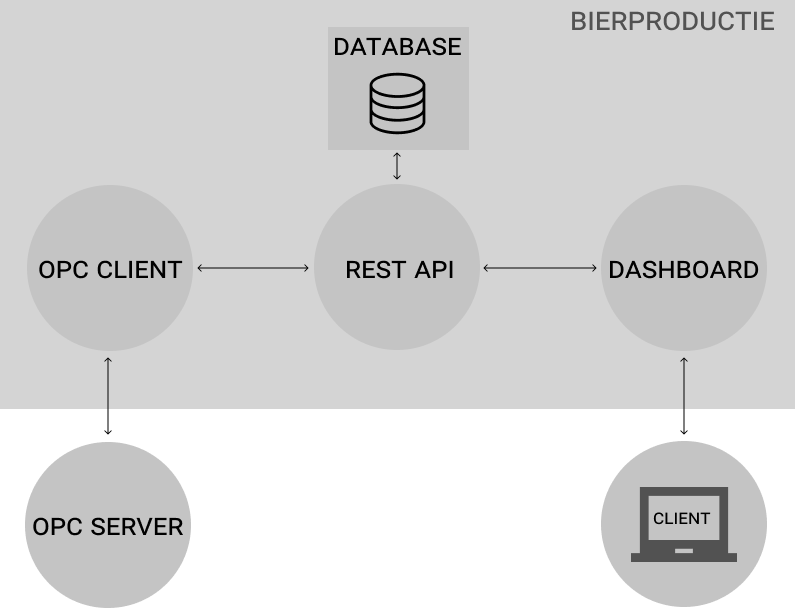
\includegraphics[scale=0.4]{images/system_overview.png}
\label{figure:bierproductie_system}
\end{figure}

Bachelor of Engineering, Software Technology\\
\vspace{2mm}
Semesterproject 3. semester, ST3-PRO\\
\vspace{2mm}
\textbf{Project Period:} 31.08.2020 - 14.12.2020 \\
\vspace{2mm}
\textbf{Hand in date:} 14.12.2020 \\

\vspace{7mm}

\textbf{Group 06:} \\
\vspace{2mm}
Jakob Rasmussen, jakra19@student.sdu.dk \\
\vspace{2mm}
Kenneth M. Christiansen kechr19@student.sdu.dk \\
\vspace{2mm}
Kevin K. M. Petersen, kepet19@student.sdu.dk \\
\vspace{2mm}
Kristian N. Jakobsen, kjako19@student.sdu.dk \\
\vspace{2mm}
Simon Jørgensen, sijo819@student.sdu.dk \\

\vspace{7mm}

\textbf{Supervisor:} Parisa Niloofar, parni@mmmi.sdu.dk \\

% Bottom of page
\vfill

University of Southern Denmark \\
The Faculty of Engineering \\
The Mærsk Mc-Kinney Møller Institute \\
Campusvej 55, 5230 Odense M 

\end{center}
\end{titlepage}

    \newpage
    
    \begin{tabular}{@{}l l} 
\textbf{Title:} & Bierproductie \\
& \\
\textbf{Institution:} & University of Southern Denmark \\
& The Faculty of Engineering, The Mærsk Mc-Kinney Møller Institute \\
& Campusvej 55, 5230 Odense M \\
& \\
\textbf{Education:} & Bachelor of Engineering, Software Technology\\
& \\
\textbf{Semester:} & 3. Semester \\
& \\
\textbf{Course Title:} & Industrial 4.0 cyber-physical software systems \\
& \\
\textbf{Internal Course Code:} & ST3-PRO \\
& \\
\textbf{Project Period:} &  31.08.2020 - 19.12.2020\\
& \\
\textbf{ECTS:} & 10 ECTS\\
& \\
\textbf{Supervisor:} & Parisa Niloofar\\
& \\
\textbf{Project group:} & 06\\
& \\

\\
\end{tabular}

% VARIABLES
\newcounter{PROD}
\setcounter{PROD} {1}

%%%%


% Jakob Jakob Jakob Jakob Jakob Jakob Jakob Jakob Jakob Jakob Jakob
\ifnum \value{PROD}=1
    
\includegraphics[scale=0.07]{images/signatures/signatureJR.jpg}
    \vspace{-9.5mm}
\fi
\par\rule{\textwidth}{0.4pt}

Jakob Rasmussen, jakra19@student.sdu.dk\\
% -end- -end- -end -end -end- -end- -end -end -end- -end- -end -end -end-

% Kenneth Kenneth Kenneth Kenneth Kenneth Kenneth Kenneth Kenneth Kenneth

\ifnum \value{PROD}=1
    
\includegraphics[scale=0.3]{images/signatures/signature_kechr19.PNG}
    \vspace{-5mm}
\fi
\par\rule{\textwidth}{0.4pt}

Kenneth M. Christiansen, kechr19@student.sdu.dk\\
\vspace{3.5mm}
% -end- -end- -end -end -end- -end- -end -end -end- -end- -end -end -end-

% KEVIN KEVIN KEVIN KEVIN KEVIN KEVIN Kevin Kevin Kevin Kevin Kevin Kevin
\vspace{-6.5mm}

\ifnum \value{PROD}=1
    
\includegraphics[scale=0.3]{images/signatures/signature_kepet19.png}
    \vspace{-8mm}
\fi
\par\rule{\textwidth}{0.4pt}

Kevin K. M. Petersen, kepet19@student.sdu.dk
% -end- -end- -end -end -end- -end- -end -end -end- -end- -end -end -end-

% Kristian Kristian Kristian Kristian Kristian Kristian Kristian

\ifnum \value{PROD}=1
    
\includegraphics[scale=0.04]{images/signatures/signature_kjako19.jpg}
    \vspace{-9.5mm}
\fi
\par\rule{\textwidth}{0.4pt}

Kristian N. Jakobsen, kjako19@student.sdu.dk\\
% -end- -end- -end -end -end- -end- -end -end -end- -end- -end -end -end-

% Simon Simon Simon Simon Simon Simon Simon Simon Simon Simon Simon Simon

\ifnum\value{PROD}=1
    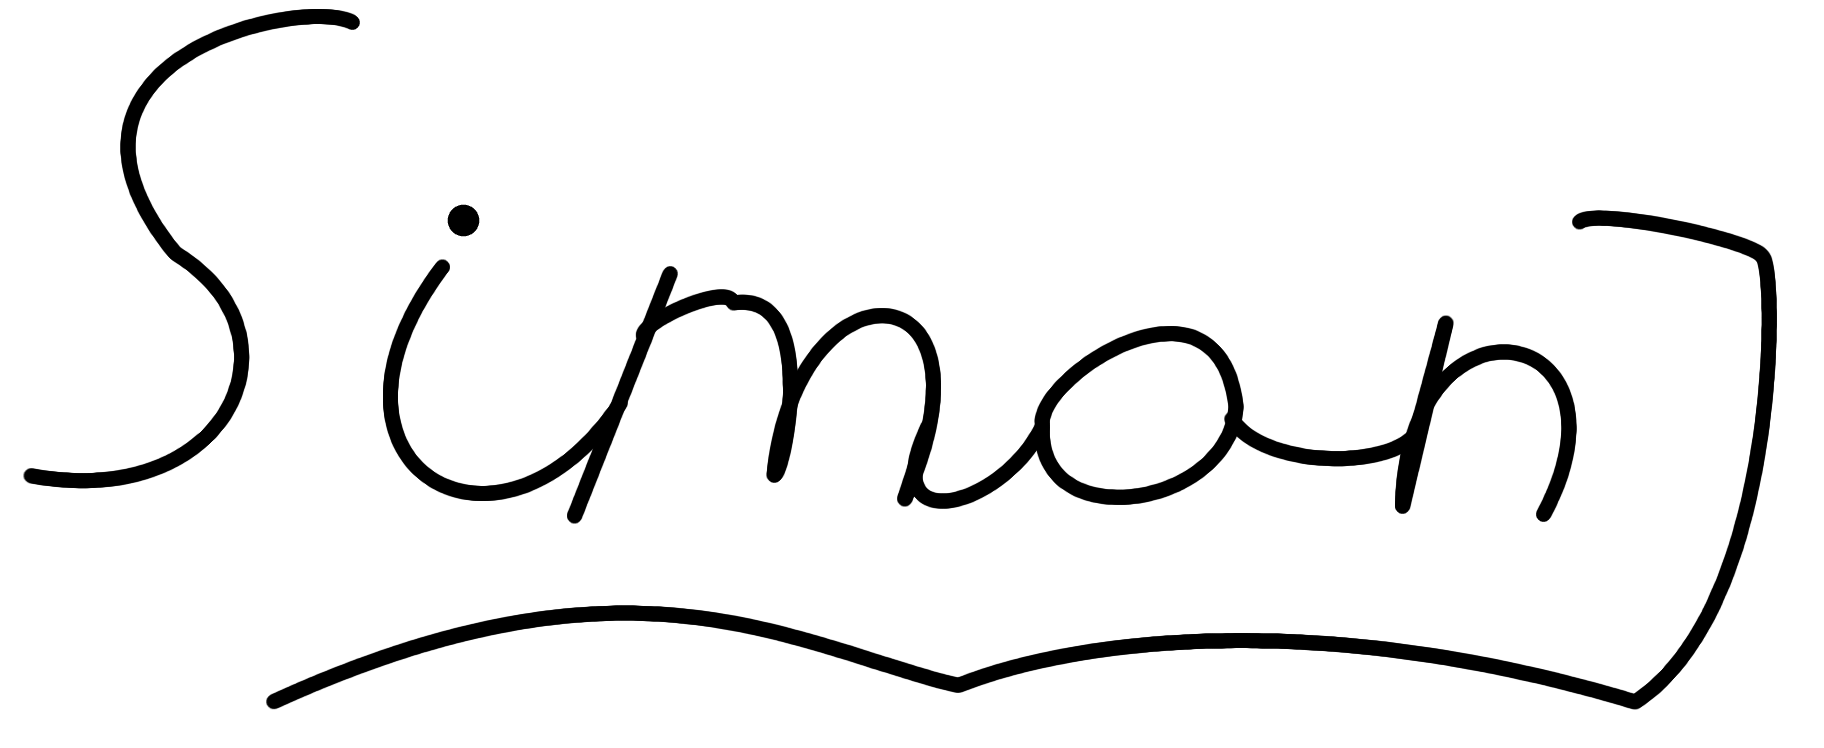
\includegraphics[scale=0.042]{images/signatures/signatureSJ.png}
    \vspace{-3.5mm}
\fi
\par\rule{\textwidth}{0.4pt}

Simon Jørgensen, sijo819@student.sdu.dk\\
% -end- -end- -end -end -end- -end- -end -end -end- -end- -end -end -end-

%Bottom of page
%\vfill

\begin{tabular}{@{}l l}
Pages:      & 21 \myworries{Remember me :)} \\
Appendix:   & 0 \myworries{And me! :)}
\end{tabular}

\vspace{3.5mm}

\begin{footnotesize}

\textbf{By signing this document, each group member confirms that everyone have participated equally to this project, and everyone is thus collectively responsible for the content of the report.}
\end{footnotesize}

    \newpage

    \section{Summary}
The purpose of this project has been to develop an MES for the brewery
Refslevbæk Bryghus A/S, to optimise the production line so the brewery
can keep up with the demand. The brewery recently bought a new brewing machine,
and a simulator of this has been made available to the group. An initial
requirements analysis of the project case has been made and based on this, the
group has narrowed the problem down to the following:\\

\textit{"How to apply an MES to control and optimise the brewing process at
Refslevbæk Bryghus A/S, to maximise the production of high-quality beer."}\\

During the development phase, the group has made use of the framework Scrum, to
organise the group work. A meeting has been held every week, to plan the next
step in the development process as well as make issues for the planned tasks.
These issues are assigned to a two-week sprint. To manage this, the management
solution, ZenHub, has been used alongside GitHub. For each task, an issue has
been created and a group member has been assigned. \\

The group has managed to develop an MES consisting of a dashboard, an API and an
OPC-UA Client. The dashboard acts as a control panel, from which a beer batch
can be started and stopped, the machine can be cleared and reset. Real-time data
is displayed, which the user can interact with in order to see detailed graphs.
A history page can be accessed, containing data regarding past batches. The data
is stored in a database and is used for batch reports and further analysis. The
stored data is also used to further optimise the production line, for example by
calculating the Overall Equipment Effectiveness (OEE). The REST API is used as a
translator between the dashboard and the OPC-UA client.
    \newpage

    \setcounter{tocdepth}{2} % anything below subsection will not be added
    \section{Table of Contents}

    \newpage

    \section{Editorial}
In Table \ref{table:editorial}, the people who were responsible for each section
are listed.
\begin{table}[ht]
    \begin{tabularx}{\textwidth}{|>{\RaggedRight}X|>{\RaggedRight}X|>{\RaggedRight}X|>{\RaggedRight}X|}
        \hline
        \textbf{Section} & \textbf{Responsible} & \textbf{Collaborator} & \textbf{Checked}\\
        \hline
        Frontpage & \textit{N/A} & \textit{N/A} & \textit{N/A}\\
        \hline
        Titlepage & \textit{N/A} & \textit{N/A} & \textit{N/A}\\
        \hline
        Summary & Kenneth & Jakob & \textit{N/A}\\
        \hline
        Editorial & Jakob & \textit{N/A} & \textit{N/A}\\
        \hline
        List of Figures & Kenneth & \textit{N/A} & \textit{N/A}\\
        \hline
        List of Tables & Kenneth & \textit{N/A} & \textit{N/A}\\
        \hline
        Introduction & Kristian & \textit{N/A} & \textit{N/A}\\
        \hline
        Theory \& Methods & Kenneth, Jakob & \textit{N/A} & \textit{N/A}\\
        \hline
        Requirements & Jakob & Kenneth & \textit{N/A}\\
        \hline
        Analysis & Kenneth & Simon, Jakob & \textit{N/A}\\
        \hline
        Architecture & Kenneth & \textit{N/A} & \textit{N/A}\\
        \hline
        Design & Kenneth & Kevin, Jakob & \textit{N/A}\\
        \hline
        Implementation & Kristian, Simon, Kevin, Kenneth & \textit{N/A} & \textit{N/A}\\
        \hline
        Verification \& Validation & Simon & \textit{N/A} & \textit{N/A}\\
        \hline
        Evaluation & Kevin & \textit{N/A} & \textit{N/A}\\
        \hline
        Conclusion & Jakob, Kenneth, Kevin, Kristian, Simon & \textit{N/A} & \textit{N/A}\\
        \hline
        Appendix & Kevin & \textit{N/A} & \textit{N/A}\\
        \hline
    \end{tabularx}
    \caption{Editorial} 
    \label{table:editorial}
\end{table} 
    \newpage
    
    \section{List of Figures}

    \newpage
    
    % Start counting from this line
    \pagenumbering{arabic}
    \setcounter{page}{1}

    \renewcommand{\thesection}{\arabic{section}} 
    \renewcommand{\thesubsection}{\thesection.\arabic{subsection}}
    \setcounter{section}{0}

    \section{Introduction}

% Motivation from project proposal
As students, this semester project gives the group great learning experience as
well as a good idea of how such a project would progress. During the project,
the group will learn how to create and set up an Open Platform Communications
Unified Architecture, OPC-UA, client, and how to make it communicate directly
to a physical machine. The group will learn to host a web server, from which the
machine can be controlled, and access it as a website. The group will also have
the chance to learn and use a new scripting language, JavaScript. The gained
experience is the main motivation of this project.

% Problem formulering
\subsection{Problem Statement}
In the table \ref{table:problem-statement}, the finished problem, the problem statement and related questions are listed.
\begin{table}[ht]
    \begin{tabularx}{\textwidth}{|>{\RaggedRight}p{4cm}|>{\RaggedRight}X|}
        \hline
        \textbf{Problem} & The current production line is not effecient enough to keep up with the demand of the beer, while still maintaining a quality product\\
        \hline
        \textbf{Problem Statement} & How to control and optimise the brewing machine, to maximise the production of high quality beer\\
        \hline
        \textbf{Related questions} & 
            \begin{itemize}
                \item How can we optimise the production?
                \item How can we utilise calculus and linear algebra to provide a meaningful overview of the production line, based on statistics?
                \item How can we create a web based frontend for the MES?
                \item How can we separate the different aspects of the system (separation of concerns)
            \end{itemize}
        \hline
    \end{tabularx}
    \caption{Problem statement showcase} 
    \label{table:problem-statement}
\end{table} 

% Overview of project
\subsection{Overview of project}
This project aims to improve the beer machine by increasing quantity while 
maintaining quality. To accomplish this the project will offer an interactive 
web interface for monitoring, controlling and adjusting the brewery machine. 
This is done by having the web interface interact with a REST API that connects 
to a client. This client controls the machine through an OPC-UA server 
connection and stores relevant data in a database.

    \newpage

    \section{Background}
    \newpage

    \section{Problem analysis}

    \newpage

    \section{Theory \& Methods}
\subsection{Theory}

\subsubsection{Overall Equipment Effectiveness}
The \textbf{O}verall \textbf{E}quipment \textbf{E}ffectiveness, OEE, is a
measurement of how effective a given production line is. It identifies what
percentage of the manufacturing time that is truly productive. The formula for
the OEE can be seen in equation \ref{eq:OEE}
\begin{equation} \label{eq:OEE}
    OEE = \frac{Good Count * Ideal Cycle Time}{Planned Produciton Time}
\end{equation}

Where \textit{Good Count} is the amount of acceptable products produced,
\textit{Ideal Cycle Time} is the theoretical minimum time to produce a single
product and \textit{Planned Production Time} is the total time that the
manufacturing process is scheduled for production.

\subsection{Methods}
\subsubsection{Scrum}
To keep track of the group work, the Scrum framework, with a few exceptions, is
used. Scrum consists of multiple artefacts and ceremonies, and in this project
product roadmap, Scrum meetings, product and sprint backlogs and burndown charts
will be used. Each sprint will have a duration of two weeks and the issues for
the sprint backlog will be chosen at the beginning of each sprint, at the Scrum
meeting. The Scrum meeting will take place each Friday and will be a mixture of
sprint planning, daily Scrum, and sprint review. To manage Scrum, ZenHub, a
management solution that can be integrated with GitHub, is used. On ZenHub the
group will create the roadmap, that acts as a schedule for the project and
board, which is where the issues will be handled. A burndown chart for each
sprint is automatically generated and kept up to date by ZenHub. The board will
consist of five columns, as seen below.

\begin{table}[H]
    \begin{tabularx}{\textwidth}{|>{\RaggedRight}X|>{\RaggedRight}X|>{\RaggedRight}X|>{\RaggedRight}X|>{\RaggedRight}X|>{\RaggedRight}X|>{\RaggedRight}X|}
        \hline                             
        \textbf{Product Backlog} & \textbf{Sprint Backlog} & \textbf{In Progress} & \textbf{Review/QA} & \textbf{Closed} \\
        \hline
        Issues & Issues for the given sprint & Issues that is currently being worked on & Issues that are pending (or in) review & Approved issues that have been merged    \\
        \hline
    \end{tabularx}
    \caption{Scrum Board} 
    \label{table:scrum}
\end{table} 

\subsubsection{MoSCoW}
MoSCoW is an important prioritising model used in software development, as it
describes which parts of the system that constitute the minimal viable product,
MVP. The use cases for the system to be developed are prioritised with the
costumer as this makes it clear which parts of the system to develop first.
These use cases are then presented in a table, to improve readability.\\

MoSCoW is an acronym standing for:\\

\begin{description}
    \item [Must have:] the use cases needed for the system to work and be
    accepted by the customer.

    \item [Should have:] what use cases the customer would like to have
    implemented, but they are not necessarily important for the system to work.

    \item [Could have:] use cases the customer would like to have implemented if
    there is enough time for it.

    \item [Won't have (this time):] use cases that is not to be prioritised in
    this iteration, but maybe in future releases.
\end{description}

\subsubsection{FURPS+}
FURPS+ is a model for classifying functional and non-functional requirements and
help giving a detailed description of the requirements. The acronym stands for:

\begin{description}
    \item [Functionality:] What the customer wants, including security measures.

    \item [Usability:] How effective is the product from the user's point of
    view? Is the product aesthetically acceptable? Is the documentation adequate?

    \item [Reliability:] What is the most acceptable system downtime? Are system
    errors predictable? Is it possible to demonstrate how accurate the results
    are? How is the system restored?

    \item [Performance:] How fast should the system be? What is the maximum
    response time? What is the throughput? How much memory does the system use?

    \item [Supportability:] Can the system be tested? Is it possible to
    configure the system, expand it, install it, and provide service on the
    system.
\end{description}

The + sign stands for supplementary needs the customer could have, and includes:

\begin{description}
    \item [Design constraints:] Do I/O devices or database management systems
    influence how the software should be built?

    \item [Implementation requirements:] Are there any standards the programmers
    must adhere to? is test-driven development necessary?

    \item [Interface requirements:] What downstream feeds need to be made? What
    other systems should the system work with?

    \item [Physical requirements:] What hardware should the system be
    implemented on?
\end{description}
    \newpage
    
    \section{Requirements}

\subsection{Overall Requirements Specification}
\subsubsection{Summary of requirements}
The group's proposed solution will adhere to the requirements given by the
brewery Refslevbæk Bryghus A/S, which can be seen in the project description.

The manufacturing execution system, MES, must be able to control the brewery’s production.
It must be able to start and stop the production line,
as well as monitor the production and collect data from the production line.
The data must be stored for further analysis.
The MES must be able to keep track of the batches that the new machine is producing,
as well as collect various data from the machine that is associated with the current batch number.
After a finished batch production, the MES must be able to produce a batch report.
The report must contain the following.

\begin{itemize}
    \item This Batch ID
    \item Product type
    \item Amount of products (total, defect and acceptable)
    \item Amount of time used in the different states
    \item Logging of temperature over the production time
    \item Logging of humidity over the production time
\end{itemize}

The MES must be able to monitor the production and display live relevant data
from the machine. The documentation of the system must contain an illustration
that defines the different components in the setup, in relation to the
ISA88\^{}1213 Part 1 Physical Hierarchy model. The system must have a
visualisation that can be accessed and used to display production data. The
system must be able to collect the necessary data from the machine and calculate
the overall equipment effectiveness, OEE\^{}131516, of the machine. The OEE must
be available to be displayed by the system. The system must be able to estimate
the error function associated with the different products. The system must be
able to find the optimal production speed for each product type, based on an
error simulation and the appertaining graph upon which the error simulation is
built.

\subsubsection{List of requirements}
Below, in table \ref{table:Requirements}, is a list of the above requirements. These requirements have been
prioritised using the MoSCoW method, where M is for Must have, S is for
Should have, C is for could have, and W is for Won't have. 

\begin{table}[H]
    \captionof{table}{List of requirements} 
    \begin{tabularx}{\textwidth}{|>{\RaggedRight}p{1cm}|>{\RaggedRight}p{4cm}|>{\RaggedRight}X|>{\RaggedRight}p{1cm}|}
        \hline
        \textbf{ID} & \textbf{Name} & \textbf{Description} & \textbf{Prio} \\
        \hline
        R01 & Control production line & Control the brewery's production & M \\
        \hline
        R02 & Control production line & Start/stop production line & M \\
        \hline
        R03 & Monitor production & Monitor data from the production line & M \\
        \hline
        R04 & Monitor production & Store the collected data for further analysis & M \\
        \hline
        R05 & Administer batches & Keep track of produced batches (batch ID) & M \\
        \hline
        R06 & Store batch info & Collect various data associated with current batch number from the machine & M \\
        \hline
        R07 & Batch report & Produce a batch report (PDF/dashboard style format) & M \\
        \hline
        R08 & Live data & Monitor and display live relevant data from the machine & M \\
        \hline
        R09 & Documentation & Documentation must contain an illustration that defines the different components in the setup in relation to the ISA88\^{}1213 Part 1 Physical Hierarchy model & M \\
        \hline
        R10 & Visualisation & Visualisation that can be accessed and used to display the production data & M \\
        \hline
        R11 & OEE & Collect necessary data from the machine and calculate the OEE. OEE must be available to be displayed by the system & M \\
        \hline
        R12 & Estimate error function & Estimate the error function associated with the products & S \\
        \hline
        R13 & Optimal Production speed & Estimate the optimal production speed for each product type & M \\
        \hline
    \end{tabularx}
    \label{table:Requirements}
\end{table}

\subsection{Selected Detailed Requirements}

\subsubsection{Functional \& Non-Functional Requirements}
In table \ref{table:sup_requirements} you can see a description of Functional and
Non-Functional requirements. These requirements have been classified by using
the FURPS+ method.

\begin{table}[H]
    \captionof{table}{Supplementary Requirements} 
    \begin{tabularx}{\textwidth}{|>{\RaggedRight}p{5.25cm}|>{\RaggedRight}p{0.6cm}|>{\RaggedRight}X|}
        \hline
        \textbf{FURPS+}  & \textbf{\#} & \textbf{Demands} \\
        \hline
        Functionality  	& S01 & Improve the beer machine by increasing quantity while maintaining quality \\
        \hline
        Usability      	& S02 & Documentation on usage of the REST API \\
        \hline
        Reliability    	& S03 & On server reboot, the application will automatically restart \\
        \hline
        Performance    	& S04 & Max response time (API: 400 ms) \\
        \hline
        Supportability 	& S05 & Minimum browser versions (JavaScript version 6)\\
        \hline
        Design constraints 	& S06 & Na \\
        \hline
        \multirow{5}{*}{Implementation requirements} & S08 & Should be controlled via MES\\
        \cline{2-3}
                & S08 & MES should be able to keep track of Batches\\
        \cline{2-3}
                & S09 & Monitor production (Live data)\\
        \cline{2-3}
                & S10 & Estimate error function\\
        \cline{2-3}
                & S11 & Optimal production speed\\
        \hline
        \multirow{14}{*}{Interface requirements } & S12 & Show OEE \\
        \cline{2-3}
                & S13 & Show Batch Report that include:
            \begin{itemize}
                \item Batch ID
                \item Product type
                \item Amount of products (total, defect and acceptable)
                \item Amount of time used in the different states
                \item Logging of temperature over the production time
                \item Logging of humidity over the production time
            \end{itemize} \\
        \cline{2-3}
            & S14 & Visualisation \\
        \hline
        Physical requirements & S14 & The group should work with the beer 
        production machine provied by SDU \\
        \hline
    \end{tabularx}
    \label{table:sup_requirements}
\end{table} 

\subsection{Use Cases}
Use cases are written descriptions of how a user will perform different tasks
on a system. They outline a systems behaviour as it responds to a request from
the user. Each use case is represented as a sequence of steps, beginning with
the users goal and ending it when that goal is fulfilled. \\

The first step in developing use cases is to determine the actors.


% \begin{table}[ht]
%    \begin{tabularx}{\textwidth}{|>{\RaggedRight}p{3cm}|>{\RaggedRight}X|>{\RaggedRight}p{2.5cm}|}
%     \hline
%     \textbf{Use Case ID}   & \textbf{Name}                                 & \textbf{Definition}\\ \hline
%     UC01                   & Start production line                         & User \\ \hline
%     UC02                   & Stop production line                          & User \\ \hline
%     UC03                   & Monitor and store data from production line   & SCADA \\ \hline
%     UC04                   & Monitor and display relevant data live        & SCADA \\ \hline
%     UC05                   & Create batch report                           & MES \\ \hline
%     UC06                   & Calculate OEE                                 & MES \\ \hline
%     UC07                   & Estimate the error function                   & MES \\ \hline
%     UC08                   & Find optimal production speed                 & MES \\ \hline
%     \end{tabularx}
%     \caption{Use Cases}
%     \label{table:use_cases}
%     \end{table}

\subsubsection{Actor List}
In order to determine who will be able to access the system, the actors are
found. An actor is defined as any external system or user that communicates
with the system. Not every actor can necessarily be found at the given time,
meaning other actors may be found later during development.

The identified actors can be seen in table \ref{table:actor_list}. With these
actors, a visualisation can be made, depicting how the different actors
communicate with the system.

\begin{table}[H]
    \captionof{table}{Actor list}
     \begin{tabularx}{\textwidth}{|>{\RaggedRight}p{2.5cm}|>{\RaggedRight}p{8cm}|>{\RaggedRight}X|}
     \hline
     \textbf{Actor} 				& \textbf{Description}                                                                                                              				& \textbf{Goal} \\ \hline
     \multirow{2}{*}{User (p)}      & The user represents the worker of the machine. The user will use the control panel to control the machine.                                  		& 	\begin{itemize}
     																																														\item Control machine
     																																														\item Start new batches
     																																													\end{itemize} \\ \hline
     \multirow{2}{*}{BPM (s)}     	& The beer production machine is responsible for supplying data to the MES and producing the beer.       											& \begin{itemize} 
     																																														\item Collect and save data
     																																														\item Communicate between hardware and MES 
     																																									 				\end{itemize} \\ \hline
    \end{tabularx}
    \label{table:actor_list}
\end{table}

\subsubsection{Detailed Use Cases}
When the actors have been determined, use cases can be developed. These use
cases add value because they help explain how the system behaves and which
functions to include when developing the system. As seen below, in table
\ref{table:usecase_start}, which represents the sequence of steps happening
when a user wants to start the beer production machine. This use case clarifies
the functions needed to fulfil the users goal, to start the production machine.
The remaining detailed use cases can be seen in appendix \ref{app:usecases}.

% start production
\begin{table}[H]
    \captionof{table}{Production Control: Start machine}
    \begin{tabularx}{\textwidth}{|>{\RaggedRight}X|}
        \hline
        \textbf{ID:} UC01  \\
        \hline
        \textbf{Primary actor:} The user \\
        \hline
        \textbf{Secondary actor:} Beer production machine \\
        \hline
        \textbf{Short description:} The MES must be able to start the brewery's
        production \\
        \hline
        \textbf{Pre conditions:} The beer production machine needs to be in
        ready mode, that is, not producing beer. \\
        \hline
        \textbf{Main flow:} \\
        	1. This use case starts when a user wants to start the beer
        	production machine. \\
        	2. The user chooses what kind of beer to be produced. \\
        	3. The user sets production speed. \\
        	4. The user sets batch id. \\
        	5. The user sets amount of beers to be produced. \\
        	6. The user presses the start button. \\
        	7. The MES starts the machine. \\
        	8. When the production has finished, the MES stores data from the
        	production. \\

		\hline
        \textbf{post conditions:} The beer production machine is turned on \\
        \hline
        \textbf{Alternative flow:} \\
        	Step 8: If the machine does not complete the production (for various
        	reasons) the production stops and stores the data from the machine
        	and the user receives an error message. \\
        \hline
    \end{tabularx}
    \label{table:usecase_start}
\end{table}

\subsubsection{Use Case Diagram}
Below, in figure \ref{figure:ucdiagram}, an overview of the use cases for the
MES can be seen.

\begin{figure}[ht]
	\centering 
	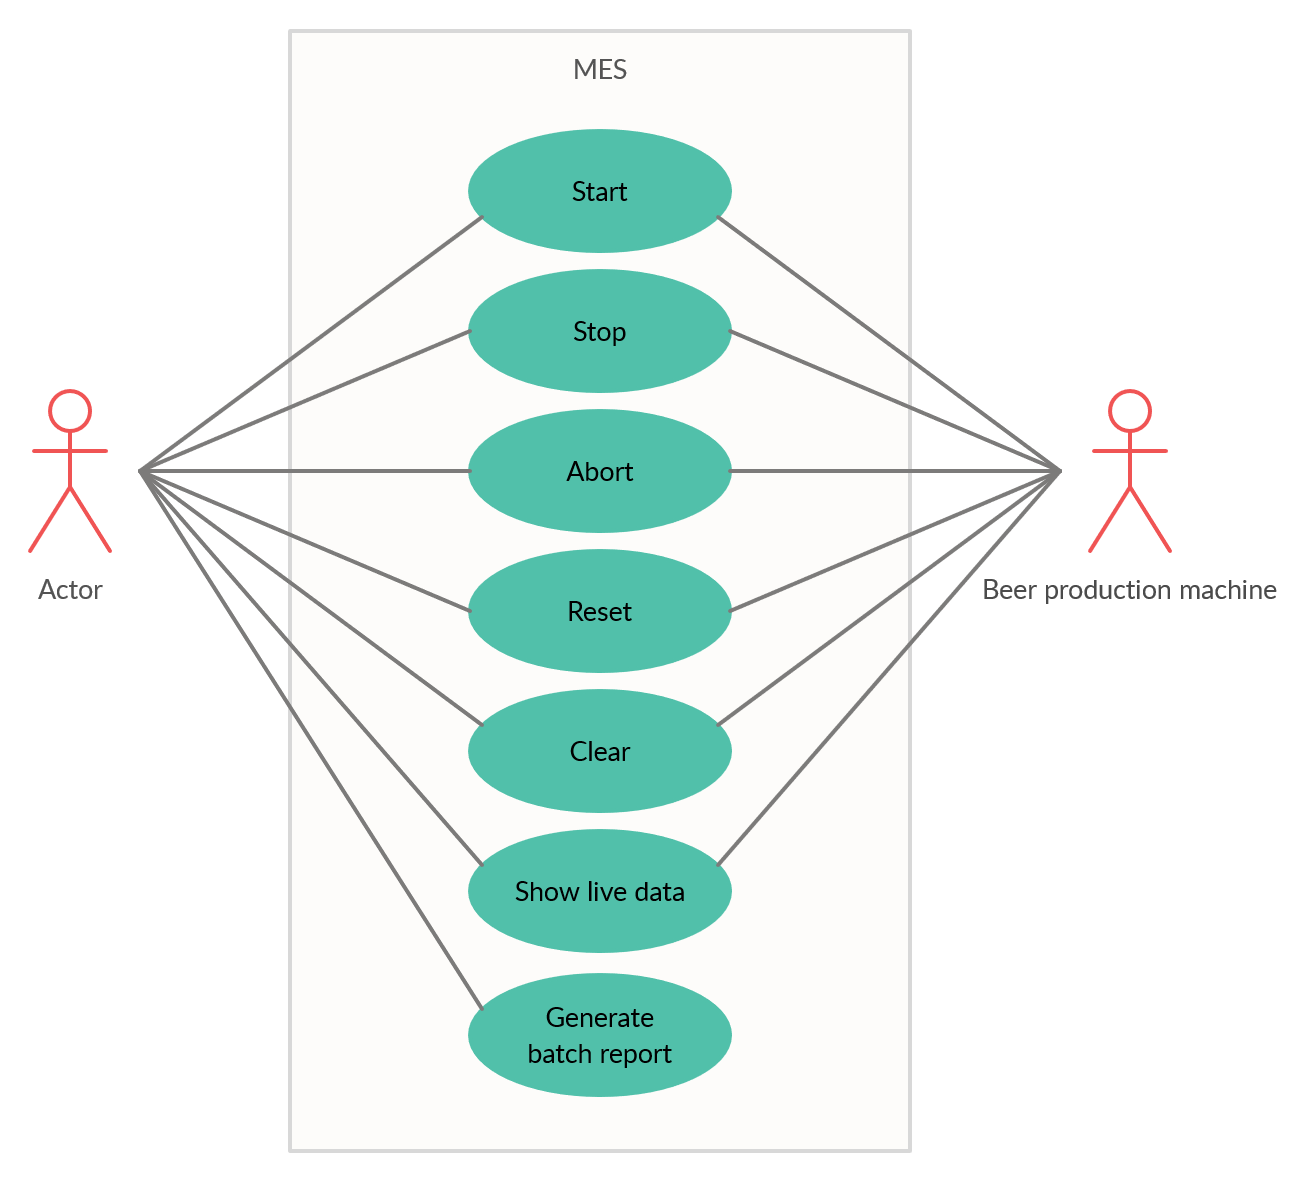
\includegraphics[scale=0.3]{images/ucdiagram.png}
	\caption{Use case diagram}
	\label{figure:ucdiagram} 
\end{figure}

    \newpage

    \section{Analysis}

\subsection{Use Case analysis}

\subsubsection{Class Candidates}

\subsubsection{Description of Classes}

\subsubsection{UML Analysis Diagram}

\subsection{Use Case Realisation}

\subsubsection{Sequence Diagrams}
A sequence diagram shows the system events for a given scenario of a use case,
and how the actor interacts with the system to solve the use case. There are two
kinds of sequence diagrams, system and operation. The system sequence diagram
displays the system as a 'black box', where the internal system events are not
shown, but only the external. This means that the diagram displays how actors
generate system events and what the system output is. Furthermore, the diagram
functions as a timeline for the system events. \\

\myworries{maybe add a system sequence diagram and explain why we used it}

The operation sequence diagram displays the system as a 'white box', where both
the internal and external system events are described, as seen in figure
\ref{figure:sequence_diagram}.

\begin{figure}[ht]
\centering 
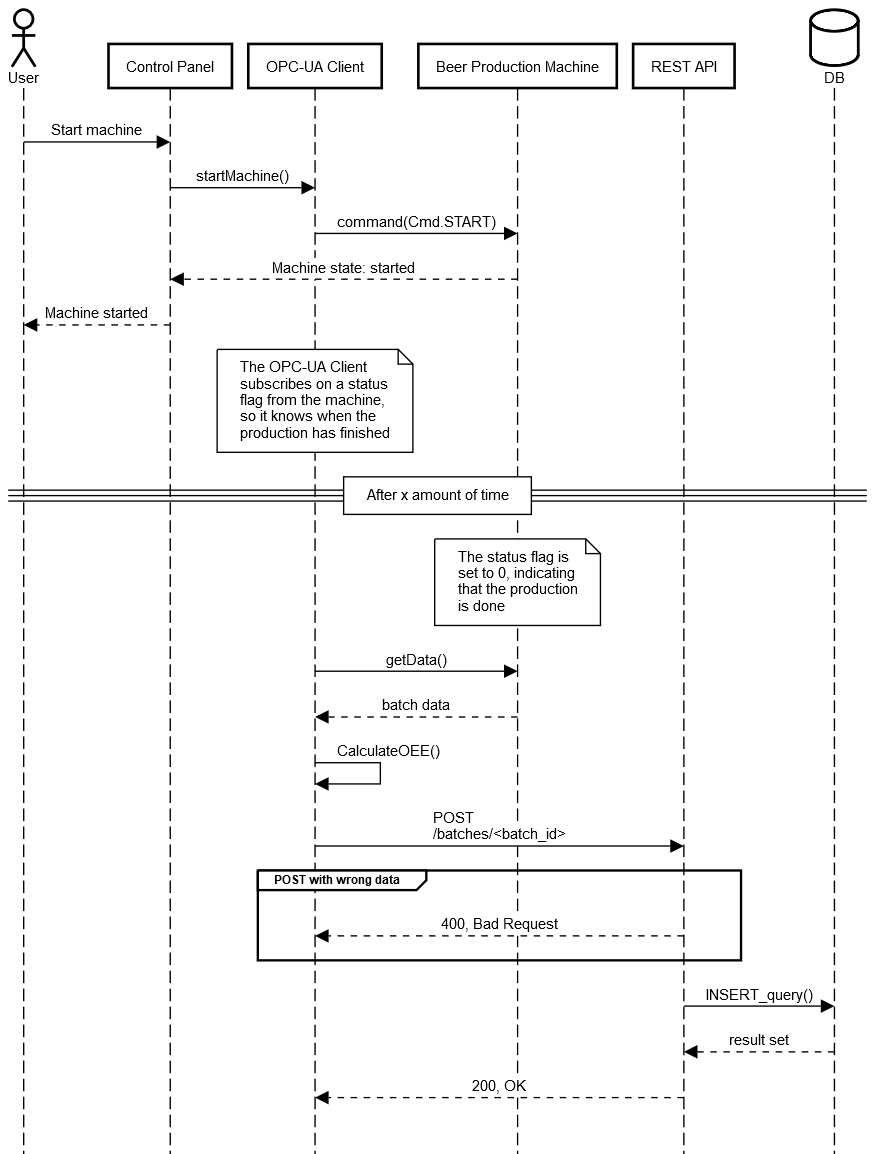
\includegraphics[scale=0.3]{images/sequence_operation/start.png}
\caption{Sequence diagram: start}
\label{figure:sequence_diagram} 
\end{figure}

This sequence diagram is used to identify system functions, as the events shown
in the diagram are the functions needed to complete the use case. In this
specific use case, the actor, the user, wants to start the beer production
machine. The user interacts with the control panel by pressing the start button,
which then sends a command to the OPC-UA client. The OPC-UA client interprets
the command as a start machine command, which triggers an event in the OPC-UA
client to send a command to the beer production machine. The beer production
machine interprets the command as a start command, which then turns on the 
machine. As a response to the user, to beer production machine sets a flag
which the control panel reacts to, and sends a message to the user. \\

When the beer production has finished, the OPC-UA client collects all relevant
data from the beer production machine. This data is used to calculate the
optimal production speed, estimate the error function, and calculate the OEE.
These calculation are used to optimise the beer production. The calculated data
and the data collected from the machine is then stored in a database. This
happens through a REST API which acts as a translator between the different 
subsystems within the MES.

\subsubsection{Operation Contracts}

\subsubsection{Updated UML Class Diagram}
\begin{figure}[ht]
\centering 
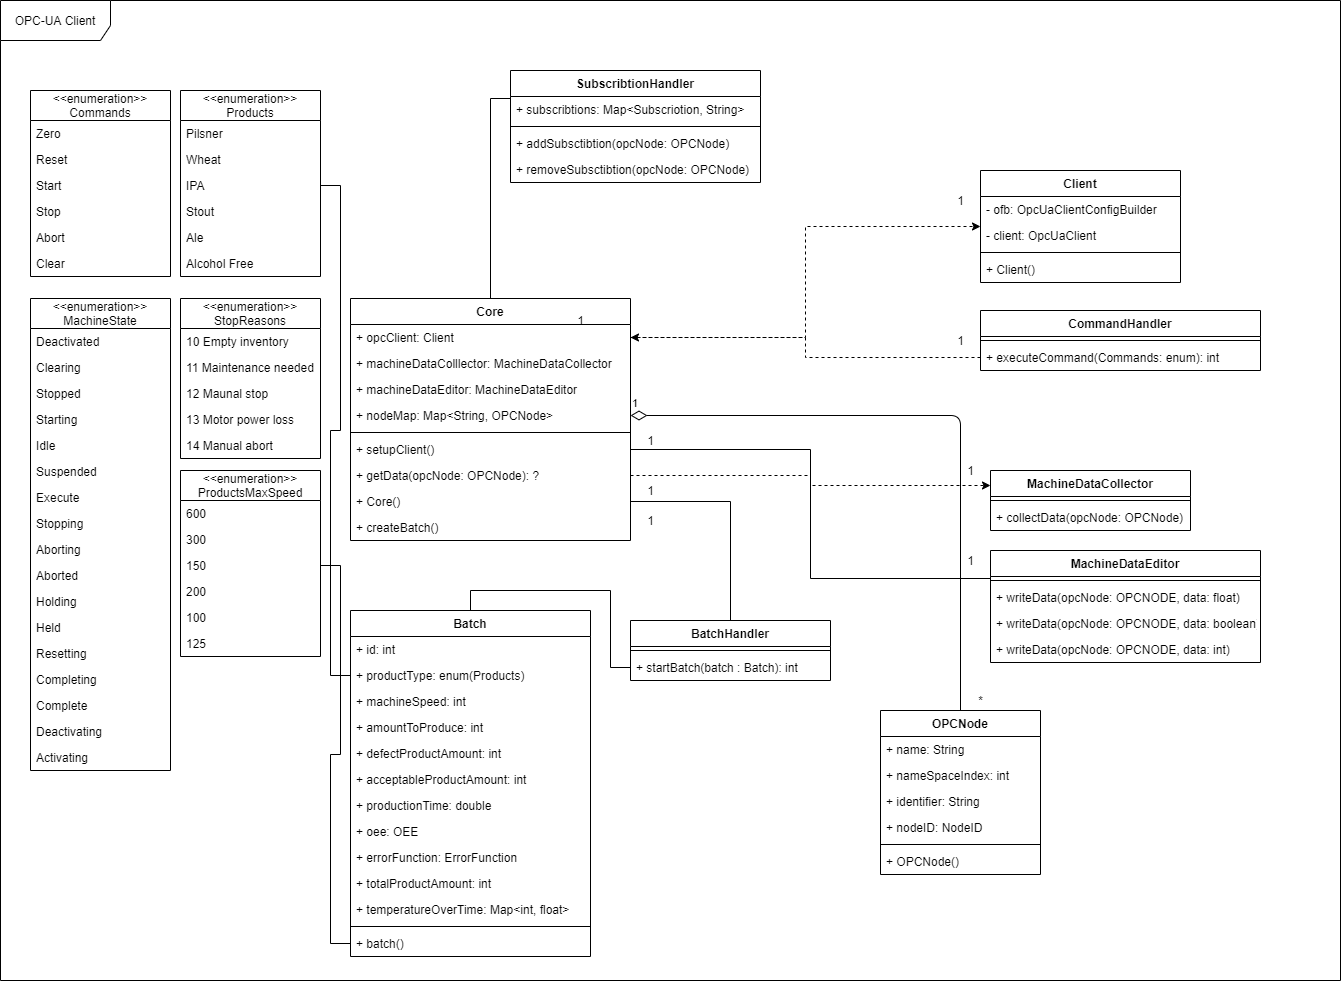
\includegraphics[scale=0.3]{images/diagrams/updated_UML_Class_Diagram.drawio.png}
\caption{Updated UML Class Diagram}
\label{figure:updated_UML_class_diagram} 
\end{figure}


The updated UML class diagram illustrates the current system idea based on the 
analysis of the system. Although this diagram only shows the 
OPC-UA client, it still gives a good idea of how this part of the system is going
to be, once implemented. \\

By using the diagram in the implementation phase, the group has a good starting 
point to expand on. The classes in the UML class diagram have a chance of not 
being implemented if the group finds them unuseful or changed to adhere to the 
program.
    \newpage

    \section{Architecture}
From the analysis of the of the project it was clear that an OPC-UA
client was needed, as this should connect to the beer production machine. This
client should in some way store the collected data from the production machine,
which means that some kind of database should be a part of the MES. As the data
would only consist of simple data types, integers, strings, etc., it was decided
to use a relational database. This way, data from different batches could easily
be stored in such a way that the relations between the data could be kept as
needed. By having a database, the subsystems do not have to store data
locally, thus making the same data available for other parts of the system,
securing data consistency. \\

It was discussed whether to develop a desktop client functioning as a dashboard
to control the production machine or if it should be a web client. The decision
landed on a web client. A web client is a more simple solution for the dashboard
as it can run in all supported web browsers. If the company then chooses to
change hardware, the dashboard is still functional. \\
 
To make the data from the database available to all subsystems in the MES, 
it was decided to develop a REST API. This API acts as a translator
between the subsystems in the MES, therefore simplifying the data management.
An example could be that the dashboard needs the data for a specific batch to
generate a batch report. Instead of having the dashboard communicate directly
with the database, a layer is added, the REST API, which both adds security and
handles the queries in a uniform way. The database then sends a query result to
the REST API which then translates the SQL to JSON for the dashboard to read
and display to the user. \\

An overview of the MES to be developed can seen in Figure
\ref{figure:architucture_diagram}.

\begin{figure}[ht]
	\centering 
	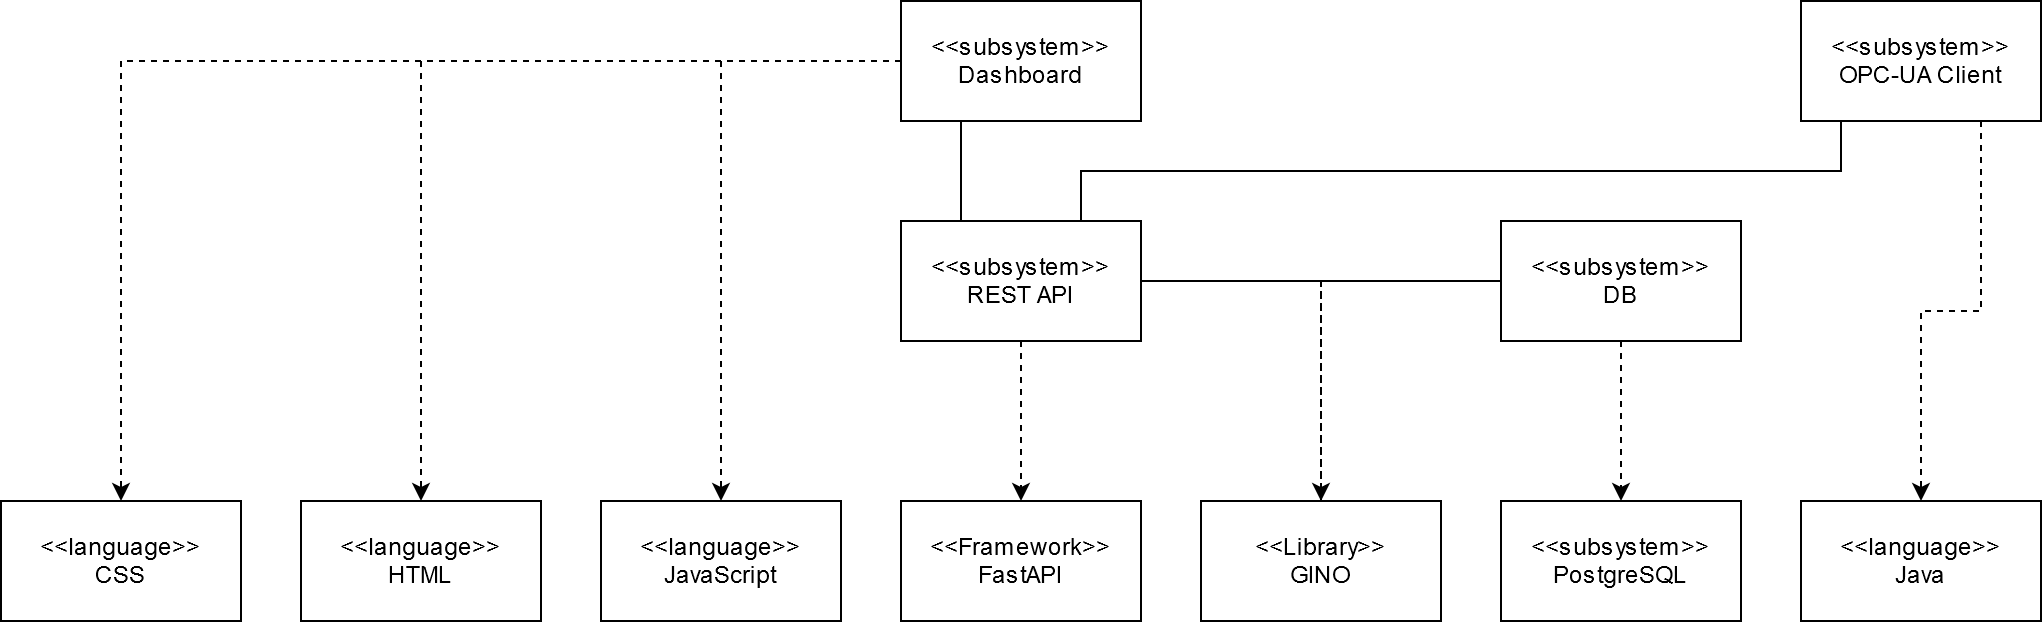
\includegraphics[scale=0.24]{images/diagrams/architecture_diagram.png}
	\caption{Software Architecture Diagram}
	\label{figure:architucture_diagram} 
\end{figure}

    \newpage

    \section{Design}

\subsection{Dashboard design}
A very important aspect the group has had to concider, is which design pattern
to model the dashboard after. A design pattern is a form of template, which in
this case, dictates how the different classes communicate. A relevant design
pattern is the MVC (Model - View - Controller). This pattern separates the
data-related logic (model), the UI logic (View) and the business logic 
(controller) into different layers, and thereby helps keep separation of
concerns. The controller manages input from the user, and forwards it to either
the model, to retrieve or store data, or the view, to present data to the user.

The group has decided to use the MVC design pattern, thus making it possible to
work on the different aspects of the system (GUI, database, logic) separately.
To ensure that these different parts of the system can communicate, a
'contract', should be created.

A visualisation of the MVC pattern can be seen in figure \ref{figure:MVC_model}

\begin{figure}[ht]
    \centering
    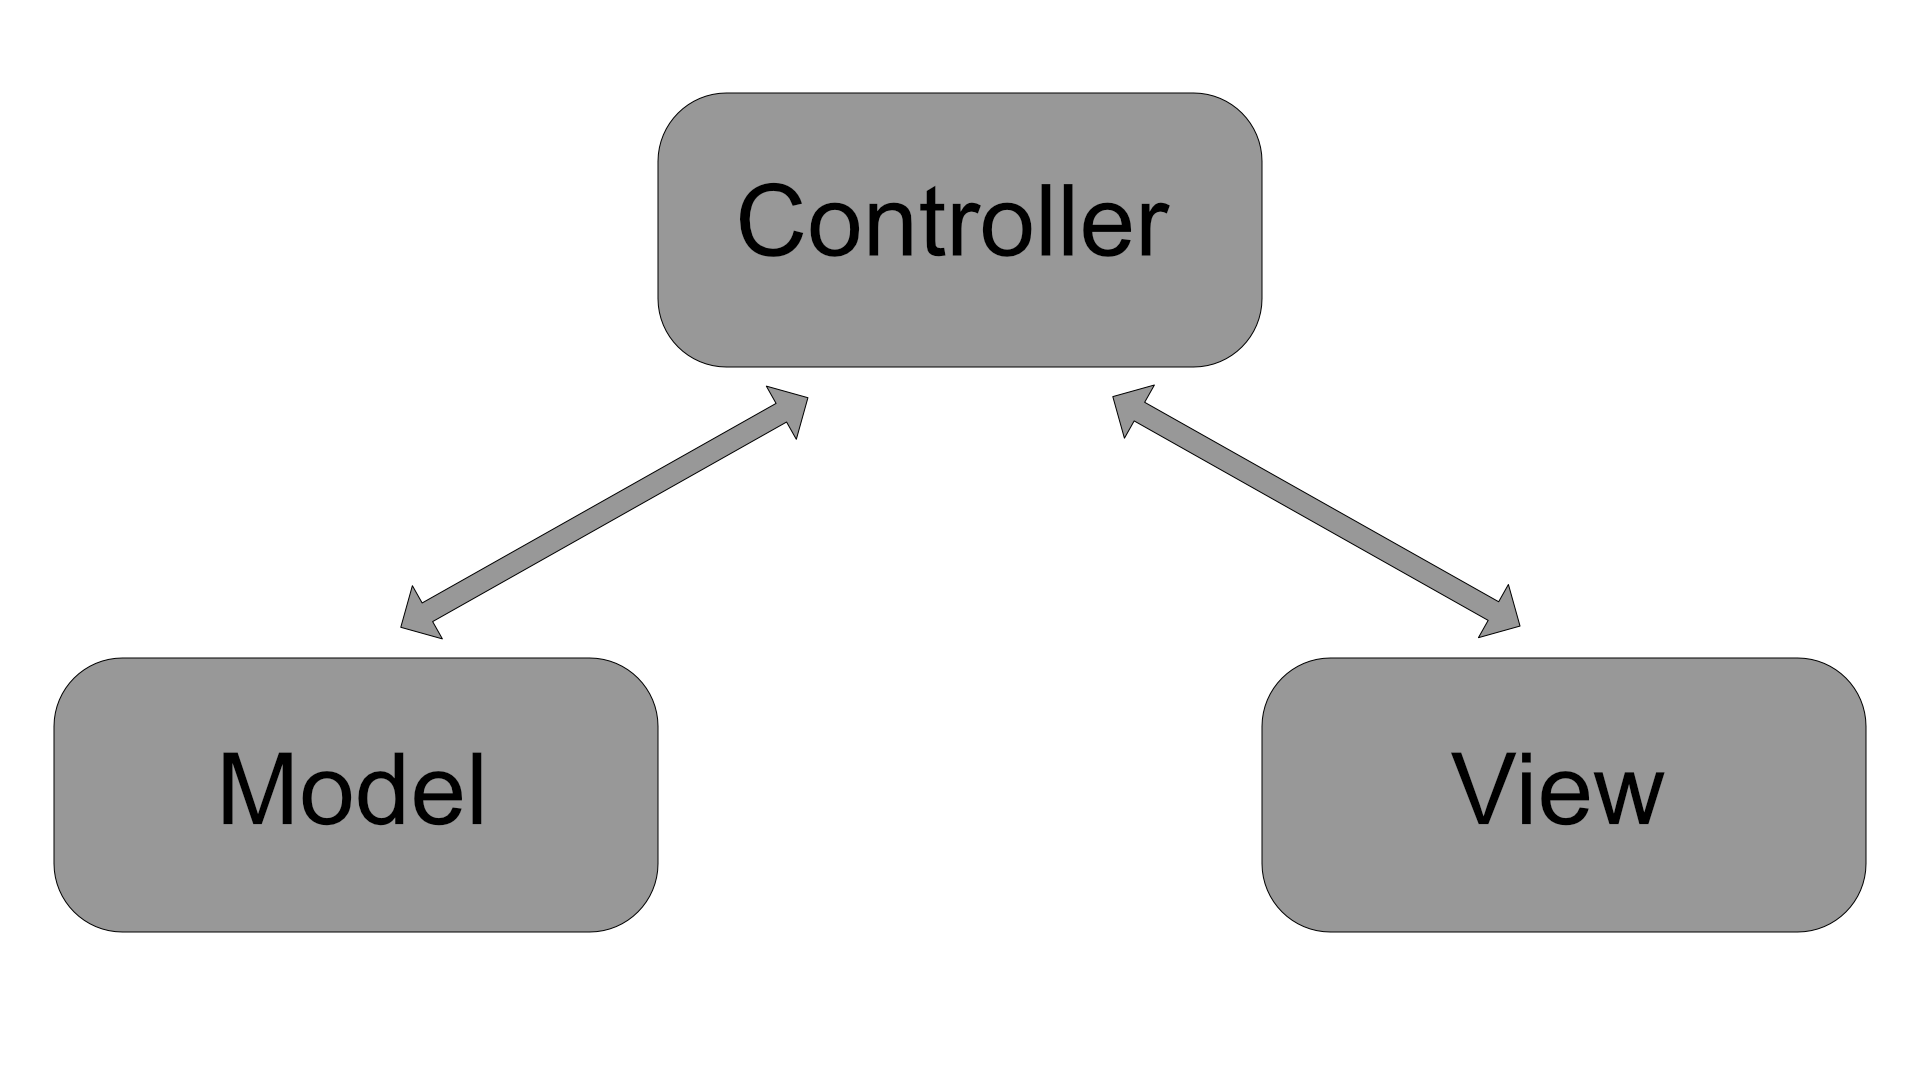
\includegraphics[scale=0.15]{images/MVC_model.png}
    \caption{MVC model}
    \label{figure:MVC_model}
\end{figure}

\subsection{Subsystem Design}
\subsubsection{OPC-UA Client}
The group was in doubt about the system being a monolith application containing 
the REST-API and OPC-UA Client in one program or split into two programs.

Choosing to split the program into two separate entities aligns with the 
separation of concerns principle fx. implementing authentication at a later 
stage(in the API) wouldn't affect the core logic of the OPC-UA client. On the 
other hand choosing to do so would add some overhead at the start of the 
implementation phase. \\

Another thing to consider when splitting the application into two separate 
entities is how they should interface with each other. To accomplish this the 
group has two options: 

\begin{table}[ht]
    \begin{tabularx}{\textwidth}{|>{\RaggedRight}X|>{\RaggedRight}X|>{\RaggedRight}X|}
        \hline
        \textbf{Option} & \textbf{Pros} & \textbf{Cons} \\
        \hline
        Console Application & Simplest to implement & Connection to the OPC-UA 
        server is created for each request (Performance overhead)\\
        \hline
        HTTP server & Connection to OPC-UA server is made once and reused. HTTP
        naturally talks JSON which is ideal as an interface & Takes longer to 
        implement \\
        \hline
    \end{tabularx}
    \caption{Options}
    \label{someLabel}
\end{table}

The group evaluated that the split up benefits outweighed the negatives. This 
decision demands that the client uses HTTP communication to communicate with the
API over localhost. 

\myparagraph{Results}
\myworries{Write after implementation}

    \newpage

    \section{Implementation}
\subsection{The Physical Setup (The Brewery Machine)}

The machine can produce different kinds of beer depending on the recipe
used. The beer is produced in batches which have their own batch id. When 
producing a batch the recipe, quantity, speed and batch id can be configured by 
an external system. When a batch has been produced the quality inspection system 
measures the quality for future use. These values are accessible in the machines 
SCADA system. The SCADA system monitors and supervises both the machines PLC 
system and the internal sensors PLC system as well as the quality inspection 
system.

\myparagraph{Sensors}
To ensure the most optimal environment beer production the 
machine is equipped with three sensors that measure the environment while 
production is happening. This data is useful as it gives insight into the 
internal environment of the machine while producing products. Currently, it 
measures temperature, humidity and vibration. The machine itself is not able to 
collect these data and are collected by an external system.

\myparagraph{Quality Inspection System}
To make it possible to calculate an error function, the system is 
equipped with a sophisticated quality inspection system. This system is key to 
optimising the production by giving data about the different error functions of 
the configurations so that they can be configured otherwise to maximise 
production. Each produced product is inspected and if the quality is low enough
the product will fail. When a batch is finished the QIS will output the amount 
of failed and passed products. The result is then used to calculate the error
function.


\subsection{The Simulator}
The group is going to use the simulator software to test the software during the
development cycle.
It is important to note that the simulator is not a replacement of the machine
since there is only so much randomness and correctness you can get from a 
simulator. 
It is still very important to have the simulator, when making prototypes and 
performing multiple tests on it, so any regressions won't be pushed to 
the production system(the beer machine).


\subsection{The dashboard}
ref to the api

\subsection{The api}
ref to the database and opc-ua

\subsection{The database}
relational yayayada postgres


\subsection{The OPC-UA-Client}
The OPC-UA-client handles the data from the machine and sends it to the API. It 
is written in java and uses the milo library to create a client that connects to 
the machines OPC-UA-server. The OPC-UA-client is able to subscribe to 
information on the server and send it to the API that stores it in the database. 
The client is also necessary to control the machine while it collects data it is 
also the client that creates and runs batches it gets from the dashboard through 
the API. It also sends live data via subscriptions, this data gets sent to the 
API every time a change appears and the API sends it to the dashboard. The 
client creates 6 subscriptions when started, they monitor temperature, 
vibration, humidity, machine-state,  current defective products and current 
processed products. 

The data gets both sent to the API and stored in an object called 
Batch. The Batch class \myworries{ref to source code I guess} has properties 
corresponding to the values the API uses as well as logic to process the data. 
This logic includes OEE calculation and JSON exportation. When running a batch a 
Batch object is created by using the data the dashboard provides. It is then run 
by providing the Batch object to the BatchHandler class that then runs the Batch 
object. While the batch is being processed the subscriptions will add data to 
the object. When done the Batch Object will run through its logic and finally 
export itself as a JSON so it can be sent to the API. 
    \newpage

    \section{Verification \& Validation}
This section describes the verification and validation of the developed MES.\\

Verification ensures the software quality, design, architecture and the like by
checking if the software has been built, according to the plan. Validation is
testing if the developed system meets the brewery's requirements found in Table
\ref{table:Requirements}.

\subsection{Verification}
The source code is compared to the results of the architecture and design
sections to verify the developed system. \\

When comparing, the focus is on ensuring that the system complies with the
design principle, separation of concerns. The database should follow the
specified EER diagram, the dashboard should comply with the design pattern MVC,
and the OPC-UA client should communicate via HTTP. \\

The database can store relevant data, and the data corresponds with the tables
specified in the EER diagram. The dashboard follows the MVC pattern, as the
Model controls the data-related logic, the View controls the user interface
logic, and the Controller controls the business logic. The OPC-UA and the REST
API are separate subsystems that communicate through the HTTP protocol. 


\subsection{Validation}
The validation tests consists of producing every product type at different
machine speeds with the same number of products to produce and gather the
production data. These tests make it possible to calculate the OEE for every
speed and then calculate the error function for the product types.\\

The validations below are concluded during the tests and list the features and
the requirements they fulfil. They also mention features that extend the basic
need of the requirements. These do not matter as much, as the ones on the list
are the primary focus. They, however, are a good addition for the overall
usability.

\subsubsection{Control production} 
The system allows control of the production line. The production manager can
start, stop, clear, reset, and abort the production through the dashboard. This
functionality fulfils requirements R01-R02 in the list of requirements.

\subsubsection{Data processing}
The system monitors batch data from the production line. The batch data is
stored in the database and kept track of, using the batch id. This functionality
allows the data to be accessed in the history page on the dashboard after it has
run, thus fulfilling requirements R03-R06.

\subsubsection{Data presentation}
Having access to past batches and their data allows the dashboard to provide a
visualisation of batch reports and live data: fulfilling requirement R07, R08,
and R9.

\subsubsection{Optimisation}
Based on past and present data, the production line can be optimised. By
calculating OEE, estimating error function and finding the optimal production
speed, the brewery can optimise their production line. These features fulfil
requirements R10-R12 completing the list of requirements. \\

By looking at the implemented features, the system fulfils the requirements from
the Overall Requirements Specification.

    \newpage

    \section{Evaluation}
The evaluation section describes how the reflections of the goals, set for the
project, meets the customer demands, as well as how the development process has
been.


\subsection{Evaluation from the customer side}
The group has managed to meet the requirements, set in the initial requirements
analysis, at the beginning of the project. The created system is able to control
the production line, using the dashboard, as well as collect, display and
store relevant data in a database. The data is used for further analysis, such
as calculating the OEE and optimal machine speed, as well as estimating the
error function.
The design of the dashboard makes it easy to see what is going on the front-page.
Every item on the front-page is there; nothing is hiding in a sub-menu.
Besides starting the beer machine, the start button would need to be pressed
to redirect the user to a start-page where a recipe, speed and the amount to
produce can be chosen. The start-page is not that convenient, because the page 
does not put in the recommended values for the different recipes, but it does
show the recommended values for the recipe.
In order to see past batches, the history page should be navigated to. This page
is easily accessible from the front-page by pressing on the button left
side menu bar. Here, past batches can be selected to inspect further. The button
layout is the same as the front-page, so there should be no learning curve there
to check out the old batches. Overall the group thinks it is a well-working
system for people not familiar with the project because it does comply with the
standard UI formalities, and there is almost no learning curve to the dashboard.


\subsection{Development process}
At the beginning of the development process, the group has held a meeting
about how the projects should be structured. Building on the experience from
last semester where Unified Process and Scrum was used, the group
decided to use both UP and Scrum again. Every Friday, a Scrum meeting is held,
to show and discuss what each group member has accomplished. Each task is
assigned to a two-week sprint, which is planned at the appropriate Scrum
meeting.
During 'matching of expectations', the group agreed upon focusing on the Minimum
Viable Product, meaning not implementing parts outside of the semester project's
scope. This has been a more realistic goal in comparison to last semester.
The use of Scrum has given a great overview of the project and has made it 
easier to plan ahead. However, looking back, the group should have scheduled 
more in the beginning. Near the end, the group has had long work hours.

The project has been divided into the four phases Unified Process; Inception,
Elaboration, Construction, and Transition. Each phase has been a fixed boundary
to plan around, making it easier to schedule, sprints, tasks, and issues.
Unlike the previous semester, no inception document was created. Instead, the
initial requirements analysis was incorporated directly into the final report.
The group could have worked more efficiently in the initial phases of Unified
Process, enabling the group to begin the Construction phase sooner.

    \newpage

    \section{Conclusion}
The group has successfully developed an MES, consisting of a dashboard, an
OPC-UA client and a REST API. The dashboard, developed using HTML, CSS, and
JavaScript, allows the user to control the production line. The OPC-UA client
connects to the beer production machine, making it possible to collect data and
control the machine by making the machine's endpoints available to the
dashboard. The client is developed in Java. The REST API, written in Python,
acts a translator between the two aforementioned subsystems as well as the
database. This allows a flow of data between the user, using the dashboard, and
the machine, using the OPC-UA client. By developing three subsystems, the MES 
complies with the design principle, separation of concerns. \\

By using calculus and linear algebra, the group has been able to provide essential
data to the brewery regarding the optimisation of their production line. This
includes estimating the error function, found in Table \ref{table:eef}, and
finding the optimal production speed, found in Table \ref{table:ops}, for each
product type, based on the overall equipment effectiveness. \\

If the brewery chooses to use the developed MES, they will be able to control
and optimise the brewing process to maximise the production of high-quality beer.
    %\newpage

    % % bibliography empty
    % \bibliographystyle{apalike}
    % % \bibliographystyle{alphabetic}
    % % \bibliographystyle{unsrt}
    % \bibliography{appendices/bibliography.bib}
    % % \medskip
    % % \printbibliography
    % \newpage
    
    % % fjerner sidetal
    % \pagenumbering{gobble}
    % % Bilag
    % \appendix % Bruges til bilag, så den laver bilag indholdfortegnelse og overskrifter
    % \input{appendices/bilag.tex}

\end{document}
